
\chapter{Conclusion}

\section{Summary}

Here we have presented a complete framework for the construction of comprehensive, high-fidelity functional maps. We have demonstrated two versions of this framework: DMS-BarSeq, a barcode-based approach that allows for high-confidence measurement of individual clones including double- and higher-order multi-mutants; and DMS-TileSeq, a fast and efficient framework that generalizes fitness effects over many different clones sharing variants of interest. Both versions use a new mutagenesis protocol, POPCode, which thanks to its accompanying webtool makes it easer than before to generate variant libraries covering the complete space of amino acid changes. At its core, the framework relies on a functional complementation assay in yeast, which can measure the overall effect of variants on protein function and has been shown to be highly predictive of variant pathogenicity in humans, outperforming common \textit{in silico} methods, despite the $\sim$ 1 billion year divergence between the two organisms. 
The DMS analysis software developed here introduces novel advances to deep mutational scanning: (i) The degree of confidence behind each measurement is carefully assessed and recorded in order to help variant classification; and (ii) variants that were missing in the complementation library or measured with low confidence were supplemented using a RandomForest-based machine learning method, yielding predictions that were found to be surprisingly reliable. 

We have evaluated the technical features of the framework on the two sumoylation pathway members UBE2I and SUMO1. We found that the functional maps generated with our method were able to successfully recapitulate known features of the proteins' biology and biochemistry and even hint at novel features that warrant further investigation. We found a large number of genetic interactions between variants in UBE2I, some of which may be due to direct compensatory relationships of amino acid replacements. Most interactions however were found to involve residue pairs separated by larger physical distances.

Having validated the framework, we demonstrated its power to detect pathogenic variants in the disease genes \gene{TPK1}, \gene{NCS1}, \gene{CALM1}, \gene{CALM2}, and \gene{CALM3}.  
We found that our Calmodulin map excelled at distinguishing disease-associated variants from benign polymorphisms and greatly outperformed the common prediction algorithms PolyPhen-2 and PROVEAN. We subsequently applied our functional map for \gene{CALM1}, \gene{CALM2}, and \gene{CALM3} to classify VUS observed in patients during gene panel sequencing and found our predictions to correlate significantly with patient indications.

\subsubsection{Limitations of the DMS framework}
Despite these successes, there are a number of limitations to the current form of our DMS framework. A fairly simple problem is the current restriction to scan relatively short genes. This is due to three reasons: (1) Longer genes would require a re-formulation of the mutagenesis protocol, as the number of mutations introduced per clone can be expected to increase linearly with gene length. This would need to be addressed by varying the concentration of mutant oligos in the amplification step. This solution could be tested systematically for templates of different lengths to determine the exact relationship between the factors involved. The results can then be added to the POPCode oligo design web tool to automatically report the most suitable protocol for each case to the experimenter.
(2) Variant clone pools for longer genes must be kept at larger population sizes at all times to avoid bottlenecking the complexity of the pools.
(3) Finally, larger libraries also require more sequencing reads to cover all variants at adequate depth. Thus they either require the use of higher-throughput instruments or would have to be processed in batches. 
A possible solution to all three problems would be to mutagenize only sections of longer genes that would be scanned separately from each other, although this would be more time consuming and costly.

A more difficult problem is that currently, the number of genes amenable to functional complementation in yeast is very limited. Song Sun and other members of the Roth lab have previously determined that only $\sim 200$ human disease genes can currently be examined using this assay~\cite{sun_extended_2016}. In addition, we found that some of these genes suffer from mapping quality issues. We observed this in the \gene{NCS1} map, which was of lower quality compared to other genes due to its relatively weak wildtype complementation fitness resulting in a less favourable signal-to-noise ratio. However it is possible that these assays might be improved by using different yeast strains with different backgrounds or by using different growth selection conditions.
Moreover, as mentioned in section~\ref{ch2discussion} of the previous chapter, we have determined that 57\% of disease genes could potentially be assayed using DMS variants based on Y2H or human cell lines instead, as will be discussed in further detail in the next section.


\section{Outlook}

\subsection{Using DMS data in a clinical context}
%DMS in clinical contexts
As introduced in chapter~\ref{ch:intro}, a major motivating factor behind the development of our framework is to address the growing problem of variants of uncertain significance observed in the clinic. While our results show that functional maps as produced by our framework can be helpful in the effort of VUS reclassification, a single line of evidence is not usually sufficient. Even though the ACMG considers functional assays among the strongest classification criteria, they require at least one additional criterium of moderate strength, such as enrichment in cases over controls, or negligible allele frequency in the general population~\cite{richards_standards_2015}. While most of the data informing the required criteria cannot be generated \textit{en masse}, other information, such as allele frequencies in the general population are available from the 1000 genomes project~\cite{the_1000_genomes_project_consortium_global_2015} and the genome and exome aggregation database (GnomAD)~\cite{lek_analysis_2016}. Thus an important goal for the future would be the construction of a public database with an underlying automatic data integration and classification system that obtains information from available sources and automatically applies the ACMG's recommended decision-making process towards variant classification. Classification results should be presented transparently, revealing the individual underlying evidence, confidence levels, and reasoning structure. 
Alternatively, it is conceivable that future iterations of DMS maps can be validated to be sufficiently rigorous to allow for a change in ACMG guidelines.

However, the commitment towards the construction of a resource is only warranted if its primary source of information, functional maps generated using Deep Mutational Scanning, can continue to be provided. The Roth lab is planning to continue building functional maps of disease genes and to expand the list of genes amenable to deep mutational scanning. A shortlist of $\sim$100 genes is planned to be addressed in the coming years. However, this undertaking is a costly one. Per 500 amino acid positions scanned, approximately \$5500 need to be spent on consumables, primarily for sequencing and oligos for POPCode mutagenesis. Assuming six genes being scanned in parallel, approximately 45 full-time employee hours need to be invested per gene. Ultimately, this undertaking cannot be shouldered by one lab alone and will require outreach to other groups. As shown in chapter~1 section~\ref{dmsIntro}, a fair number of groups are already performing deep mutational scans and may be interested in collaboration. As a first step, the Roth and Fowler labs are already collaborating with respect to mapping a number of heart disease associated genes.

\subsection{Adaptation and extentions to DMS technology}
\subsubsection{DMS in human cell lines}
As mentioned above, an important future direction is the adaptation of the deep mutational scanning framework toward directly using human cell lines in competition assays. Recent genome-wide CRISPR screens have revealed a sizable number of genes with growth phenotypes in different human cell lines~\cite{hart_high-resolution_2015,blomen_gene_2015,wang_genetic_2014}. While a number of DMS efforts have already been performed using human cells~\cite{forsyth_deep_2013,wagenaar_resistance_2014,doud_site-specific_2015,majithia_prospective_2016}, the underlying assays were not generalizable, for example, the most recent effort by Majithia and colleagues~\cite{majithia_prospective_2016} for PPAR$\gamma$ was only possible due to the fortuitous circumstances of having found a surface marker whose expression level directly reflects PPARG$\gamma$ activity. 
Atina Cote in the Roth Lab is currently working on establishing a generalizable growth-based complementation assay using CRISPR in human cell lines. 
%previous work: PPARG
%atina's CRISPR lines
%fowler's stability assay

\subsubsection{Screening of other functional elements}
Another important future direction is to expand the capability of Deep Mutational Scanning to enable assaying variants outside of protein-coding regions of the genome. However, since the space of the human genome is simply too large to be tested in its entirety the logical choice is to concentrate on elements most likely to be functionally relevant, such as splice sites, promoters, or transcription factor binding sites.
Hanane Ennajdaoui in the Roth Lab is currently working on adapting our DMS framework to scan intronic regions (shortened to exclude medial sequences).
%spliceDMS

\subsection{Other uses of DMS functional map data}

\subsubsection{Screening for viral suppressors}
Deep Mutational Scanning has many other potential uses beyond disease variant classification. As we have demonstrated in chapter~\ref{ch:data2} for \gene{UBE2I}, the method helps shed light on the biophysical mechanisms underlying the function of a gene. We have also shown that using a combination of Y2H and complementation, DMS can point to potential new protein interaction interfaces. 

UBE2I is known to be directly targeted by many viruses, such as HIV and EBV,  through specific protein-protein interactions to subvert host defenses~\cite{varadaraj_sumo_2014}. Using Y2H as the selection assay in our DMS framework and using our existing functional map of UBE2I as a reference, it would be possible to scan for variants that specifically disrupt interactions with viral proteins while not affecting overall UBE2I function. At the same time, this approach could help finding the specific interface for the interactions in question and could inform future drug development.

\begin{figure}[h!]
	\centering
	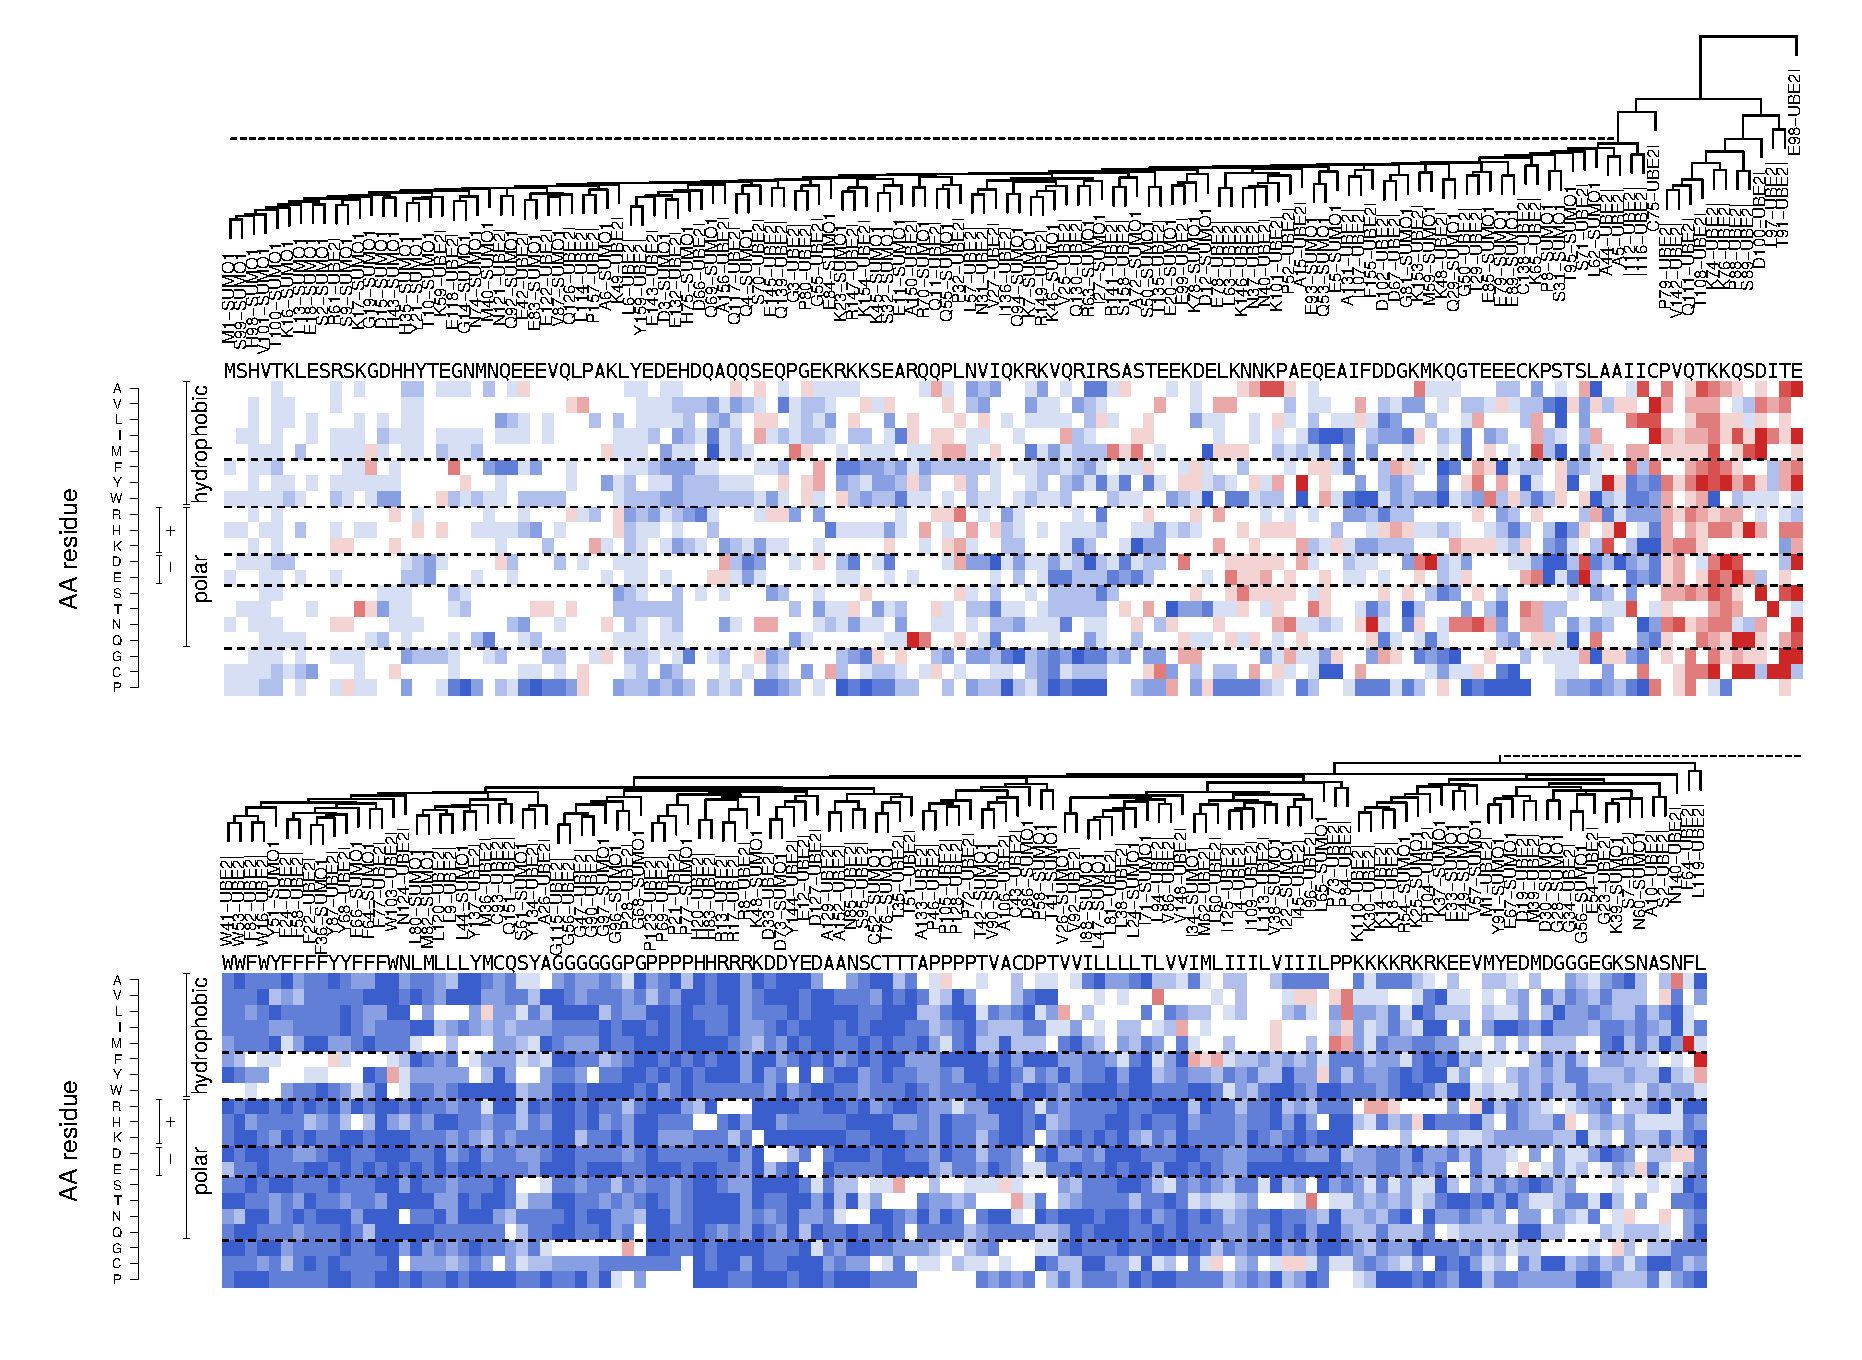
\includegraphics[width=\textwidth]{img/clustering.pdf}
	\caption{Hierarchical clustering of amino acid positions in UBE2I and SUMO1 based on mutation profile similarity}
	\label{fig:clustering}
\end{figure}

\subsubsection{Advances in computational prediction of disease variants}
As the number of functional maps produced via DMS grows, so does the its value as training data for \textit{in silico} prediction methods. Currently the number of genes scanned is not yet representative enough to cover the functional diversity of the proteome. However, Yingzhou Wu in the Roth Lab has already begun to explore its potential value for extrapolation. In an initial experiment, he was able to show that a machine learning method trained on the functional data obtained for UBE2I was able to make better predictions towards the effects of mutations in SUMO1 than if trained on the data set underlying PolyPhen-2 (HumDiv). Thus, with each new functional map added to our variant atlas, computational prediction method have the potential to become more powerful.
%  -> FUNSUM

\subsubsection{Functional classification of amino acid positions}
The same wealth of functional data that may serve as training data for future computational prediction methods may also help us learn more about the set of roles played by different residues within proteins. In an initial experiment, I have generated a hierarchical cluster map across amino acid positions in UBE2I and SUMO1 (Figure~\ref{fig:clustering}). The clustering hints at distinct functional classes occupied by different positions. There are three broad groups: (1) Positions that are generally unrestricted and can be occupied by almost any amino acid; (2) Positions that are generally constrained to a certain small number of amino acids and; (3) Positions that show hyperactivity for many possible amino acids. Within these groups there are a number of subclusters visible. For example, within the second group, certain positions only tolerate aliphatic residues, while others only tolerate aromatic residues. Evolution only samples a subset of the possible amino acids at a given position. By growing the set of proteins with complete functional maps we can potentially collect a catalog of possible functional `archetypes' for positions within proteins. Using multiple alignments we can then make predictions as to the archetype of any given position.
% -> functional classes
